\documentclass[12pt, hyperref={unicode}]{beamer}

\usepackage[T1]{fontenc}
\usepackage[utf8]{inputenc}
\usepackage[slovene]{babel}

\usepackage{pgfpages}
\usepackage{bookmark}
\usepackage{graphicx}%za vstavljanje slik
\usepackage{array}%za tabele
\usepackage{enumerate}
\usepackage{lmodern}
\usepackage{amsfonts}
\usepackage{amsmath}


\mode<presentation>

%tema
\usetheme{Berlin}
\usecolortheme{default}
\useinnertheme[shadows]{rounded}
\useoutertheme{infolines}
\setbeamertemplate{navigation symbols}{}
\beamertemplatenavigationsymbolsempty

%pisava
\usepackage{palatino}
\usefonttheme{serif}
%serif doda podaljšane črtice pri I

\newtheorem{definicija}{Definicija}
\newtheorem{izrek}{Izrek}
\newtheorem{trditev}{Trditev}
\newtheorem{posledica}{Posledica}
\newtheorem{lema}{Lema}
\newtheorem{dokaz}{Dokaz}
\newtheorem{domneva}{Domneva}


\title{(Osnovne) Igre ustvarjanja omrežja}
\subtitle{Kratka predstavitev diplome}
\author{Peter Milivojević}
\institute[FMF]{Fakulteta za matematiko in fiziko}
\date{11. \ januar \ 2024}

\begin{document}

% ===================================================================
\begin{frame}
    \titlepage
\end{frame}
% -------------------------------------------------------------------


% -------------------------------------------------------------------
\begin{frame}
   
  \frametitle{(Osnovne) Igre ustvarjanja omrežja}
  Omrežje lahko ustvarimo na več načinov in pri različnih optimizacijskih pogojih.
  Omrežje lahko ustvari centralna avtoriteta in tako doseže socialni optimum ali pa
  več sebičnih igralcev, kjer vsak poskuša doseči svoj sebični optimum v dani situaciji.
  V diplomski nalogi se bom pretežno ukvarjal z dvema verzijama osnovnih iger ustvarjanja omrežja:
  \vspace{1mm}
  \begin{itemize}
    \item Maksimalna oddaljenos
    \item Vsota oddaljenosti
  \end{itemize}

\end{frame}
% -------------------------------------------------------------------

% -------------------------------------------------------------------
\begin{frame}
   
    \frametitle{Uporabne definicije}
    \begin{definicija}
        Naj bo $G$ povezan graf in $u, v \in V(G)$. Razdalja $d(u, v)$ je dolžina najkrajše poti med vozliščema $u$ in $v$ (t.j. razdalja med $u$ in $v$) v grafu $G$.
    \end{definicija}

    \begin{definicija}
        Naj bo $G$ povezan graf. Premer grafa $G$ je definiran kot $\text{diam}(G) = \max_{u, v \in V(G)} d(u, v)$, kjer je $d(u, v)$ razdalja med vozliščema $u$ in $v$ v grafu $G$.
    \end{definicija}

    \begin{definicija}
        Naj bo $G$ povezan graf. Lokalni premer točke $v$ grafa $G$ je definiran kot $\text{diam}(G) = \max_{u \in V(G)} d(u, v)$, kjer je $d(u, v)$ razdalja med vozliščema $u$ in $v$ v grafu $G$.
    \end{definicija}

\end{frame}
% -------------------------------------------------------------------

% -------------------------------------------------------------------
\begin{frame}
   
    \frametitle{Definiciji ravnovesja}
    \begin{definicija}
       Graf je v $ravnotežju \ glede \ na \ vsoto \ razdalj$, če za vsako povezavo $vw$ in
       za vsako vozlišče $w'$ zamenjava povezave $vw$ z povezavo $vw'$ ne zmanjša
       celotne vsote razdalj od vozlišča $v$ do vseh ostalih vozlišč.
    \end{definicija}

    \begin{definicija}
        Graf je v $ravnotežju \ glede \ na \ maksimalno \ razdaljo$, če za vsako povezavo $vw$
        in za vsako vozlišče $w'$ zamenjava povezave $vw$ z povezavo $vw'$ ne zmanjša
        lokalnega premera vozlišča $v$. Nadalje odstranitev povezave $vw$ poveča
        lokalni premer vozlišča $v$.
    \end{definicija}

\end{frame}
% -------------------------------------------------------------------

% -------------------------------------------------------------------
\begin{frame}
   
    \frametitle{Kritičnost in stabilnost}  
    \begin{definicija}
        Naj bo $G$ povezan graf. Graf $G$ je $kritičen \ za \ odstranitev \ povezave$,
        če odstranitev katere koli povezave $uv \in E(G)$ poveča lokalni premer vozlišča $v$ in vozlišča $u$.
    \end{definicija}

    \begin{definicija}
        Naj bo $G$ povezan graf. Graf $G$ je $stabilen \ za \ dodajanje \ povezave$,
        če dodajanje katere koli povezave $uv \in E(G)$ ne zmanjša lokalnega premera vozlišča $v$ in vozlišča $u$.
    \end{definicija}

\end{frame}
% -------------------------------------------------------------------
  
% -------------------------------------------------------------------
\begin{frame}

  \frametitle{Drevesa: skupna vsota razdalj}
  \begin{izrek}
    Če je ravnovesni graf za skupno vsoto razdalj v preprosti igri ustvarjanja
    omrežja drevo, potem ima premer največ $2$ in je kot tak zvezda.
  \end{izrek}

  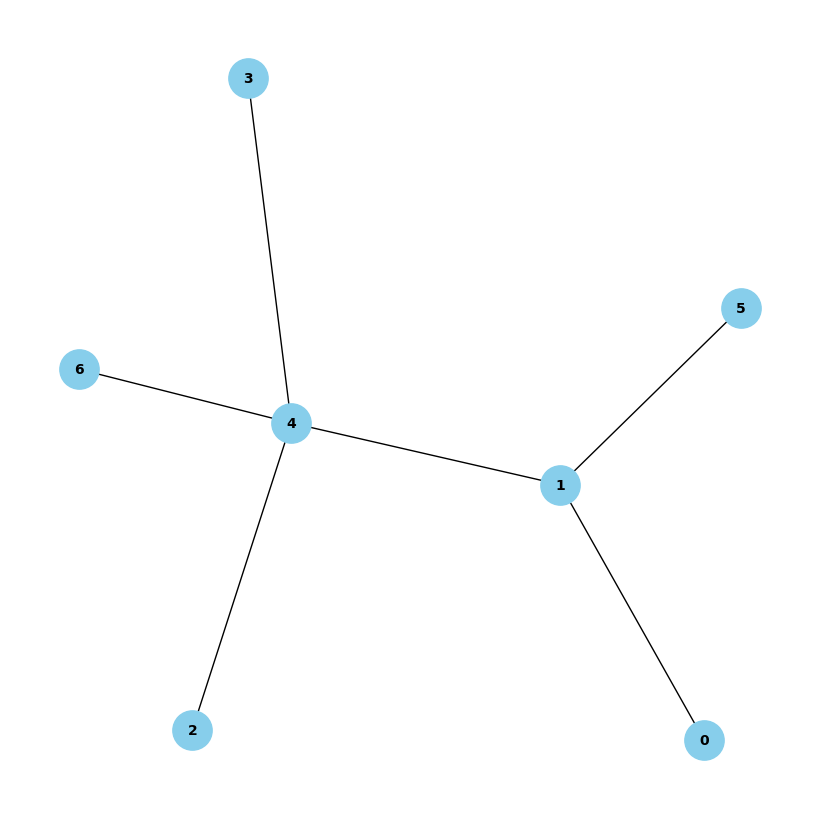
\includegraphics[width=0.3\textwidth]{drevo_1.png}
  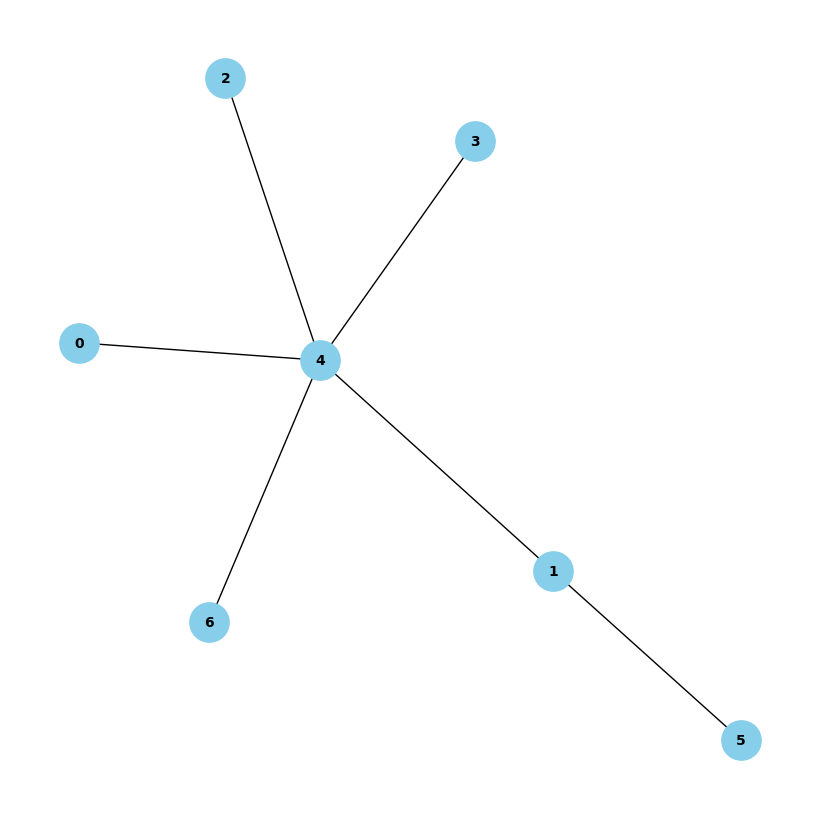
\includegraphics[width=0.3\textwidth]{drevo_2.png}
  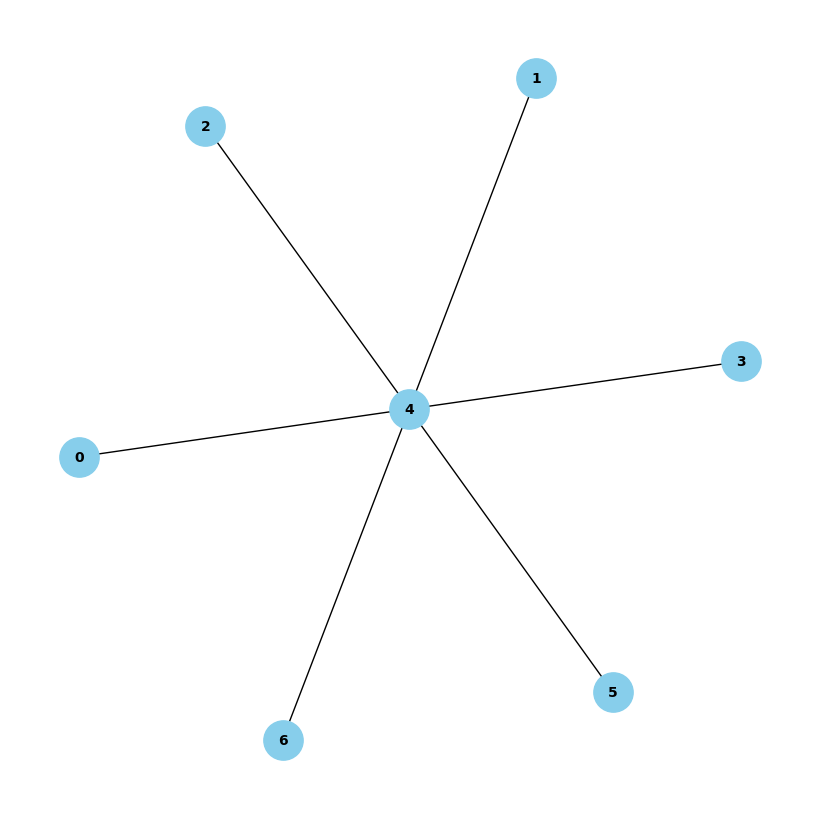
\includegraphics[width=0.3\textwidth]{drevo_3.png}
\end{frame}
% -------------------------------------------------------------------

% -------------------------------------------------------------------
\begin{frame}
   
  \frametitle{Drevesa: maksimalna razdalja}
  \begin{lema}
    V vsakem ravnovesnem grafu igre maksimalne razdalje se lokalni premer za
    katera koli $2$ poljubna vozlišča razlikuje največ za $1$.
  \end{lema}

  \begin{lema}
    Če ima ravnovesni graf za maksimalno razdaljo prerezno vozlišče, potem ima lahko
    samo ena izmed povezanih komponent $G - v$ vozlišče z razdaljo več kot $1$ od $v$.
  \end{lema}

  \begin{izrek}
    Če je ravnovesni graf za maksimalno razdaljo drevo, potem ima premer največ $3$.
  \end{izrek}

\end{frame}
% -------------------------------------------------------------------

% -------------------------------------------------------------------
\begin{frame}
  
  \frametitle{Skupna vsota razdalj: spodnje meje}
  \begin{columns}
    \column{0.5\textwidth}
    \begin{izrek}
        Obstaja ravnovesni graf za skupno vsoto razdalj s premerom 3.
      \end{izrek}
      \begin{lema}
        Za vozlišče $v$ z lokalnim premerom $2$, zamenjava sosednje povezave ne izboljša
        vsote razdalj od v.
      \end{lema}
    \column{0.5\textwidth}
    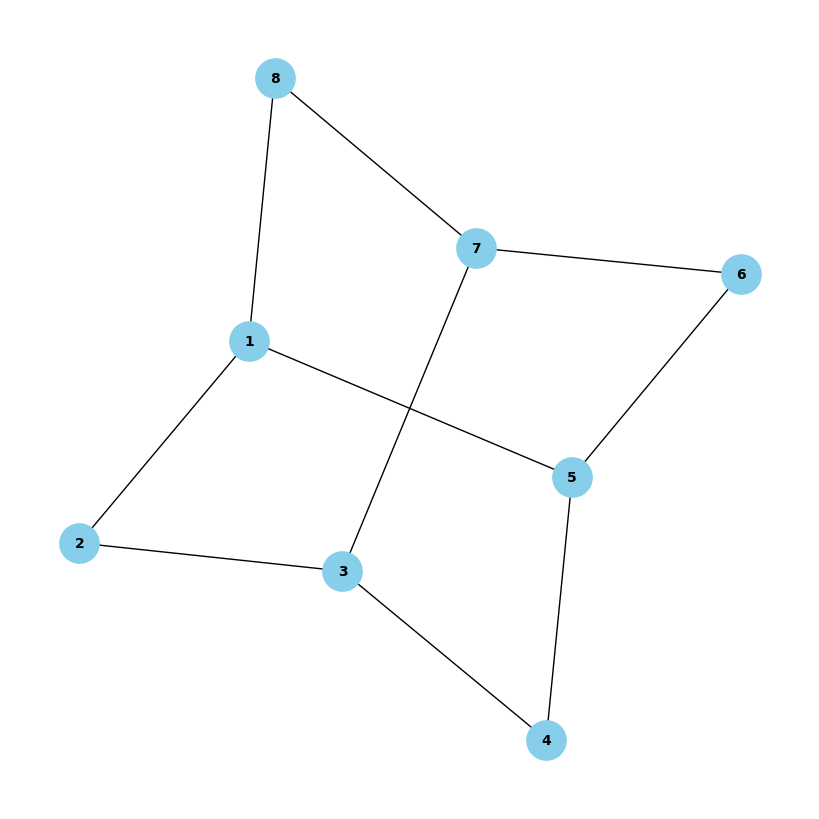
\includegraphics[width=1\textwidth]{vsota_premer_3.png}
  \end{columns}
  
\end{frame}

% -------------------------------------------------------------------

% -------------------------------------------------------------------
\begin{frame}
   
  \frametitle{Skupna vsota razdalj: zgornja meja $2^{O(\sqrt{\lg n})}$}
  \begin{izrek}
    Vsak ravnovesni graf za skupno vsoto razdalj ima premer $2^{O(\sqrt{\lg n})}$.
  \end{izrek}

  \begin{lema}
    Vsak ravnovesni graf za skupno vsoto razdalj ima premer največ $2 \lg n$ ali
    za vsako vozlišče $v$ obstaja povezava $xy$ kjer je $d(u, x) \leq \lg n$ in
    zamenjava povezave $xy$ zmanjša vsoto razdalj od $x$ za največ $2n(1 + \lg n)$.
  \end{lema}

  \begin{lema}
    V vsakem ravnovesnem grafu za skupno vsoto razdalj dodajanje poljubne povezave
    $uv$ zmanjša vsoto razdalj od $u$ za največ $5n \log n$.
  \end{lema}

\end{frame}
% -------------------------------------------------------------------

% -------------------------------------------------------------------
\begin{frame}

  \frametitle{Maksimalna razdalja}
  \begin{columns}
    \column{0.5\textwidth}
    \begin{izrek}
        Obstaja ravnovesni graf za maksimalno razdaljo z premerom $\Theta(\sqrt{n})$.
    \end{izrek}
    \column{0.5\textwidth}
    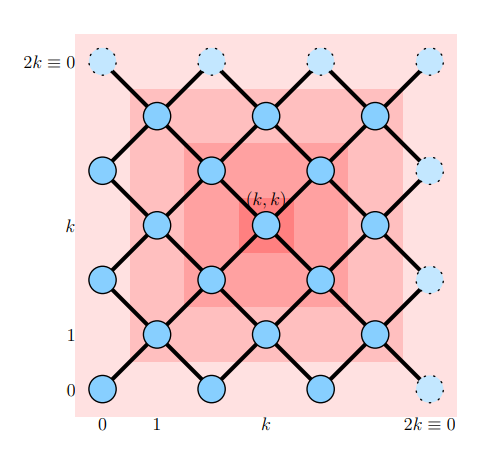
\includegraphics[width=1\textwidth]{Plagiat.png}
  \end{columns}
  
  

\end{frame}
% -------------------------------------------------------------------

% -------------------------------------------------------------------
\begin{frame}

  \frametitle{Povezava z grafi z enotsko razdaljo}
  \begin{izrek}
    Vsak ravnovesni graf za skupno vsoto razdaljo $G$ z $n \geq 24$ vozlišč in
    premerom $d > 2 \lg n$ inducira podgraf z $\epsilon\text{-skoraj-enotno-razdaljo } G'$
    z $n$ vozlišči in premerom $\Theta\left(\frac{\varepsilon d}{\lg n}\right)$ in
    podgraf z $\epsilon\text{-enotno-razdaljo } G'$ z $n$ vozlišči in premerom
    $\Theta\left(\frac{\varepsilon d}{\lg^2 n}\right)$.
  \end{izrek}

  \begin{domneva}
    Razdaljno skoraj enotni grafi imajo premer $O(\lg n)$.
  \end{domneva}


\end{frame}
% -------------------------------------------------------------------

\end{document}